\chapter{Electric Power System}
\label{ch:eps}
In this chapter, the design of the electrical power system of the \textit{Swing eVTOL} will be discussed.
Firstly, the required battery mass will be calculated in \Cref{sec:prelim_calc} to obtain the required energy to complete the mission. 
Subsequently, a general introduction to battery design and battery cells will be given in \Cref{sec:batt_cells}, discussing the elements that influence the sizing of this subsystem. 
Moreover, the complete battery pack design will be presented and justified in \Cref{sec:batt_des}, including a state of health analysis and thermal management considerations. 
Finally, in \Cref{sec:eps_concrec}, a summary of the design will be presented as well as recommendations to consider.

\section{Preliminary Calculation}
\label{sec:prelim_calc}
One of the main components during the preliminary design of an electric vehicle is the battery and power system.
To have an accurate estimate of the required battery size and weight,
it is necessary to come up with preliminary sizing methods.
Firstly, the energy required for each phase of the mission profile is computed.
After which, the total energy required for the entire mission is calculated as the following summation:

\begin{equation}
    E_\text{tot} = \sum_{0}^{m} E_{m}
\end{equation}

Having defined the energy requirement, it is now possible to compute the total battery mass needed.
To perform this calculation, it is necessary to define a new parameter, the energy density of the battery.
This can be indicated as $\rho_E$[Wh/Kg] and represents how much energy a battery can store per unit of weight.
The value of this parameter can be estimated to be \qty{300}{Wh/Kg} for state-of-the-art batteries with current technologies~\cite{stateartbat}.

Relating now the required energy and the density parameter just discussed,
it is possible to retrieve the total weight of the battery:
\begin{equation}
    w_\text{tot} = \rho_E \cdot E_\text{tot}
\end{equation}
Lastly, another fundamental quantity to take into account during a battery design is the capacity $C$.
This defines the amount of energy that can be delivered under specified conditions.
For example, if $C = \qty{100}{Ah}$, it means that a current of 100 A can be delivered for 1 hour.
To calculate the capacity, the following equation can be used:
\begin{equation}
    C_\text{pack} = \frac{w_\text{tot} \cdot \rho_E}{n_\text{pack} \cdot U_\text{ElecSys}} \label{capa}
\end{equation}
Where $n_{pack}$ is the number of battery packs, and $U_{ElecSys}$ is the nominal voltage of the system.
The calculations just shown have been performed for the initial set of requirements of 100 km of range and 200 km/h of cruise speed.
The results for both mission profiles are summarised in \Cref{tab:range_table}.

\begin{table}[htpb]
\centering
\caption{Range and battery sizing for the \textit{Swing eVTOL}}
\label{tab:range_table}
\begin{tabular}{ccc}
\toprule
\textbf{Range} {[}km{]} & \textbf{$E_\text{tot}$} {[}kWh{]} & \textbf{$m_\text{bat}$} {[}kg{]} \\
\midrule
100            & 50                   & 150                 \\
\bottomrule
\end{tabular}
\end{table}

$m_{\text{bat}}$ represents the minimum mass required to complete the mission; however, it is decided to increase the battery mass to 400 kg,
extending the range and increasing the stability characteristics of the vehicle.
This value has also been determined on the basis of the required CG shift during the transition that is required for stability. In \Cref{ch:Stability_and_Control}, it has been indeed determined that a lower total battery mass would cause the aircraft to be unstable with the current design.
Lastly, it is important to mention that a minor part of the energy stored in the battery will be converted to low-voltage current to power the avionics and other subsystems.

\section{Battery Cells}
\label{sec:batt_cells}
As the fundamental quantities defining a battery have been discussed in the previous section,
it is important to study the units that compose battery packs, the cells.
Every battery is indeed composed of single cells connected in series
and parallel to then form the final subsystem that delivers the required current and voltage.
In order to perform further calculations, firstly,
some basic parameters that belong to battery cells need to be defined:

\begin{itemize}
    \item Discharge rate (C-Rate) represents the electrical current the battery can deliver based on its capacity.
    \item State of Charge (SOC) represents the energy available in the battery.
    \item Depth of Discharge (DOD) is the energy consumed by the battery.
    \item $U_\text{nom}$ is the nominal voltage measured at a SOC of 50%.
    \item $C_\text{nom}$, nominal capacity measured at a SOC of 50%.
    \item $U_\text{c-off}$,
    also known as cut-off voltage, representing the lowest voltage limit after which the battery is considered empty.
\end{itemize}


These parameters can then be related to each other finding many dependencies.
One of the most relevant relations is between the depth of discharge and the battery voltage.
It has been proved that the cell voltages drop as the DOD increases \cite{DODGraph}.
This is a key effect to evaluate; the voltage drop leads to a drop in the maximum power that can be delivered.
Thus, the battery needs to be sized to comply with the power requirements in every flight phase.
The latter described effect is caused by the internal resistances of the battery due to electrochemical interactions
resulting in voltage-drops, according to Ohm’s law.
\Cref{fig:battery_circuit} gives a visual representation of the equivalent circuit representing this process.

\begin{figure}[H]
    \centering
    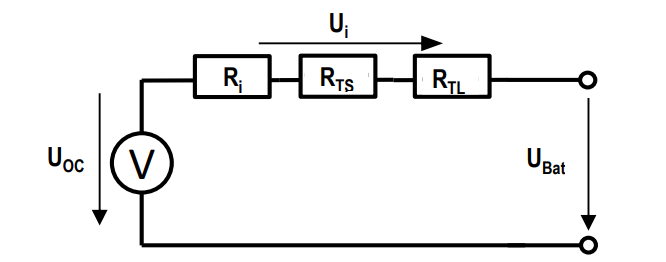
\includegraphics[width=0.5\linewidth]{figures/Battery_Circuit}
    \caption{Equivalent circuit of a battery cell discharge model}
    \label{fig:battery_circuit}
\end{figure}

In \Cref{fig:battery_circuit}, the different internal resistances are represented, but they can be simplified to one total resistance.
This reduces the calculation of the total battery voltage to: \todo{R\_e is not defined}
\begin{equation}
    U_\text{bat} = U_\text{oc} - R_{e_\text{tot}}\cdot I
\end{equation}
With $R_{e_\text{tot}}$ being the internal voltage. In \cite{DODGraph}, an extensive study on the battery discharge process has been conducted, and empirical relations between the internal resistances and the state of charge have been found that are listed below. Due to these equations, the voltage as a function of DOD has been obtained and plotted in \Cref{fig:vvsdod}.

\begin{equation} 
    U_\text{oc} = -1.031 \cdot \text{e}^{-35 \cdot \text{SOC}} + 0.321 \cdot \text{SOC}^3 + 0.1178 \cdot \text{SOC}^2 + 0.2156 \cdot \text{SOC} + 3.685
\end{equation}
\begin{equation}
        R_i = 0.1562 \cdot \text{e}^{-24.37 \cdot \text{SOC}} + 0.07446
\end{equation}
\begin{equation}
    R_\text{TS} = 0.3208 \cdot \text{e}^{-29.14 \cdot \text{SOC}} + 0.04669
\end{equation}
\begin{equation}
        R_\text{TL} = 6.6030 \cdot \text{e}^{-155.2 \cdot \text{SOC}} + 0.04984
\end{equation}


    \begin{figure}[H]
    \centering
    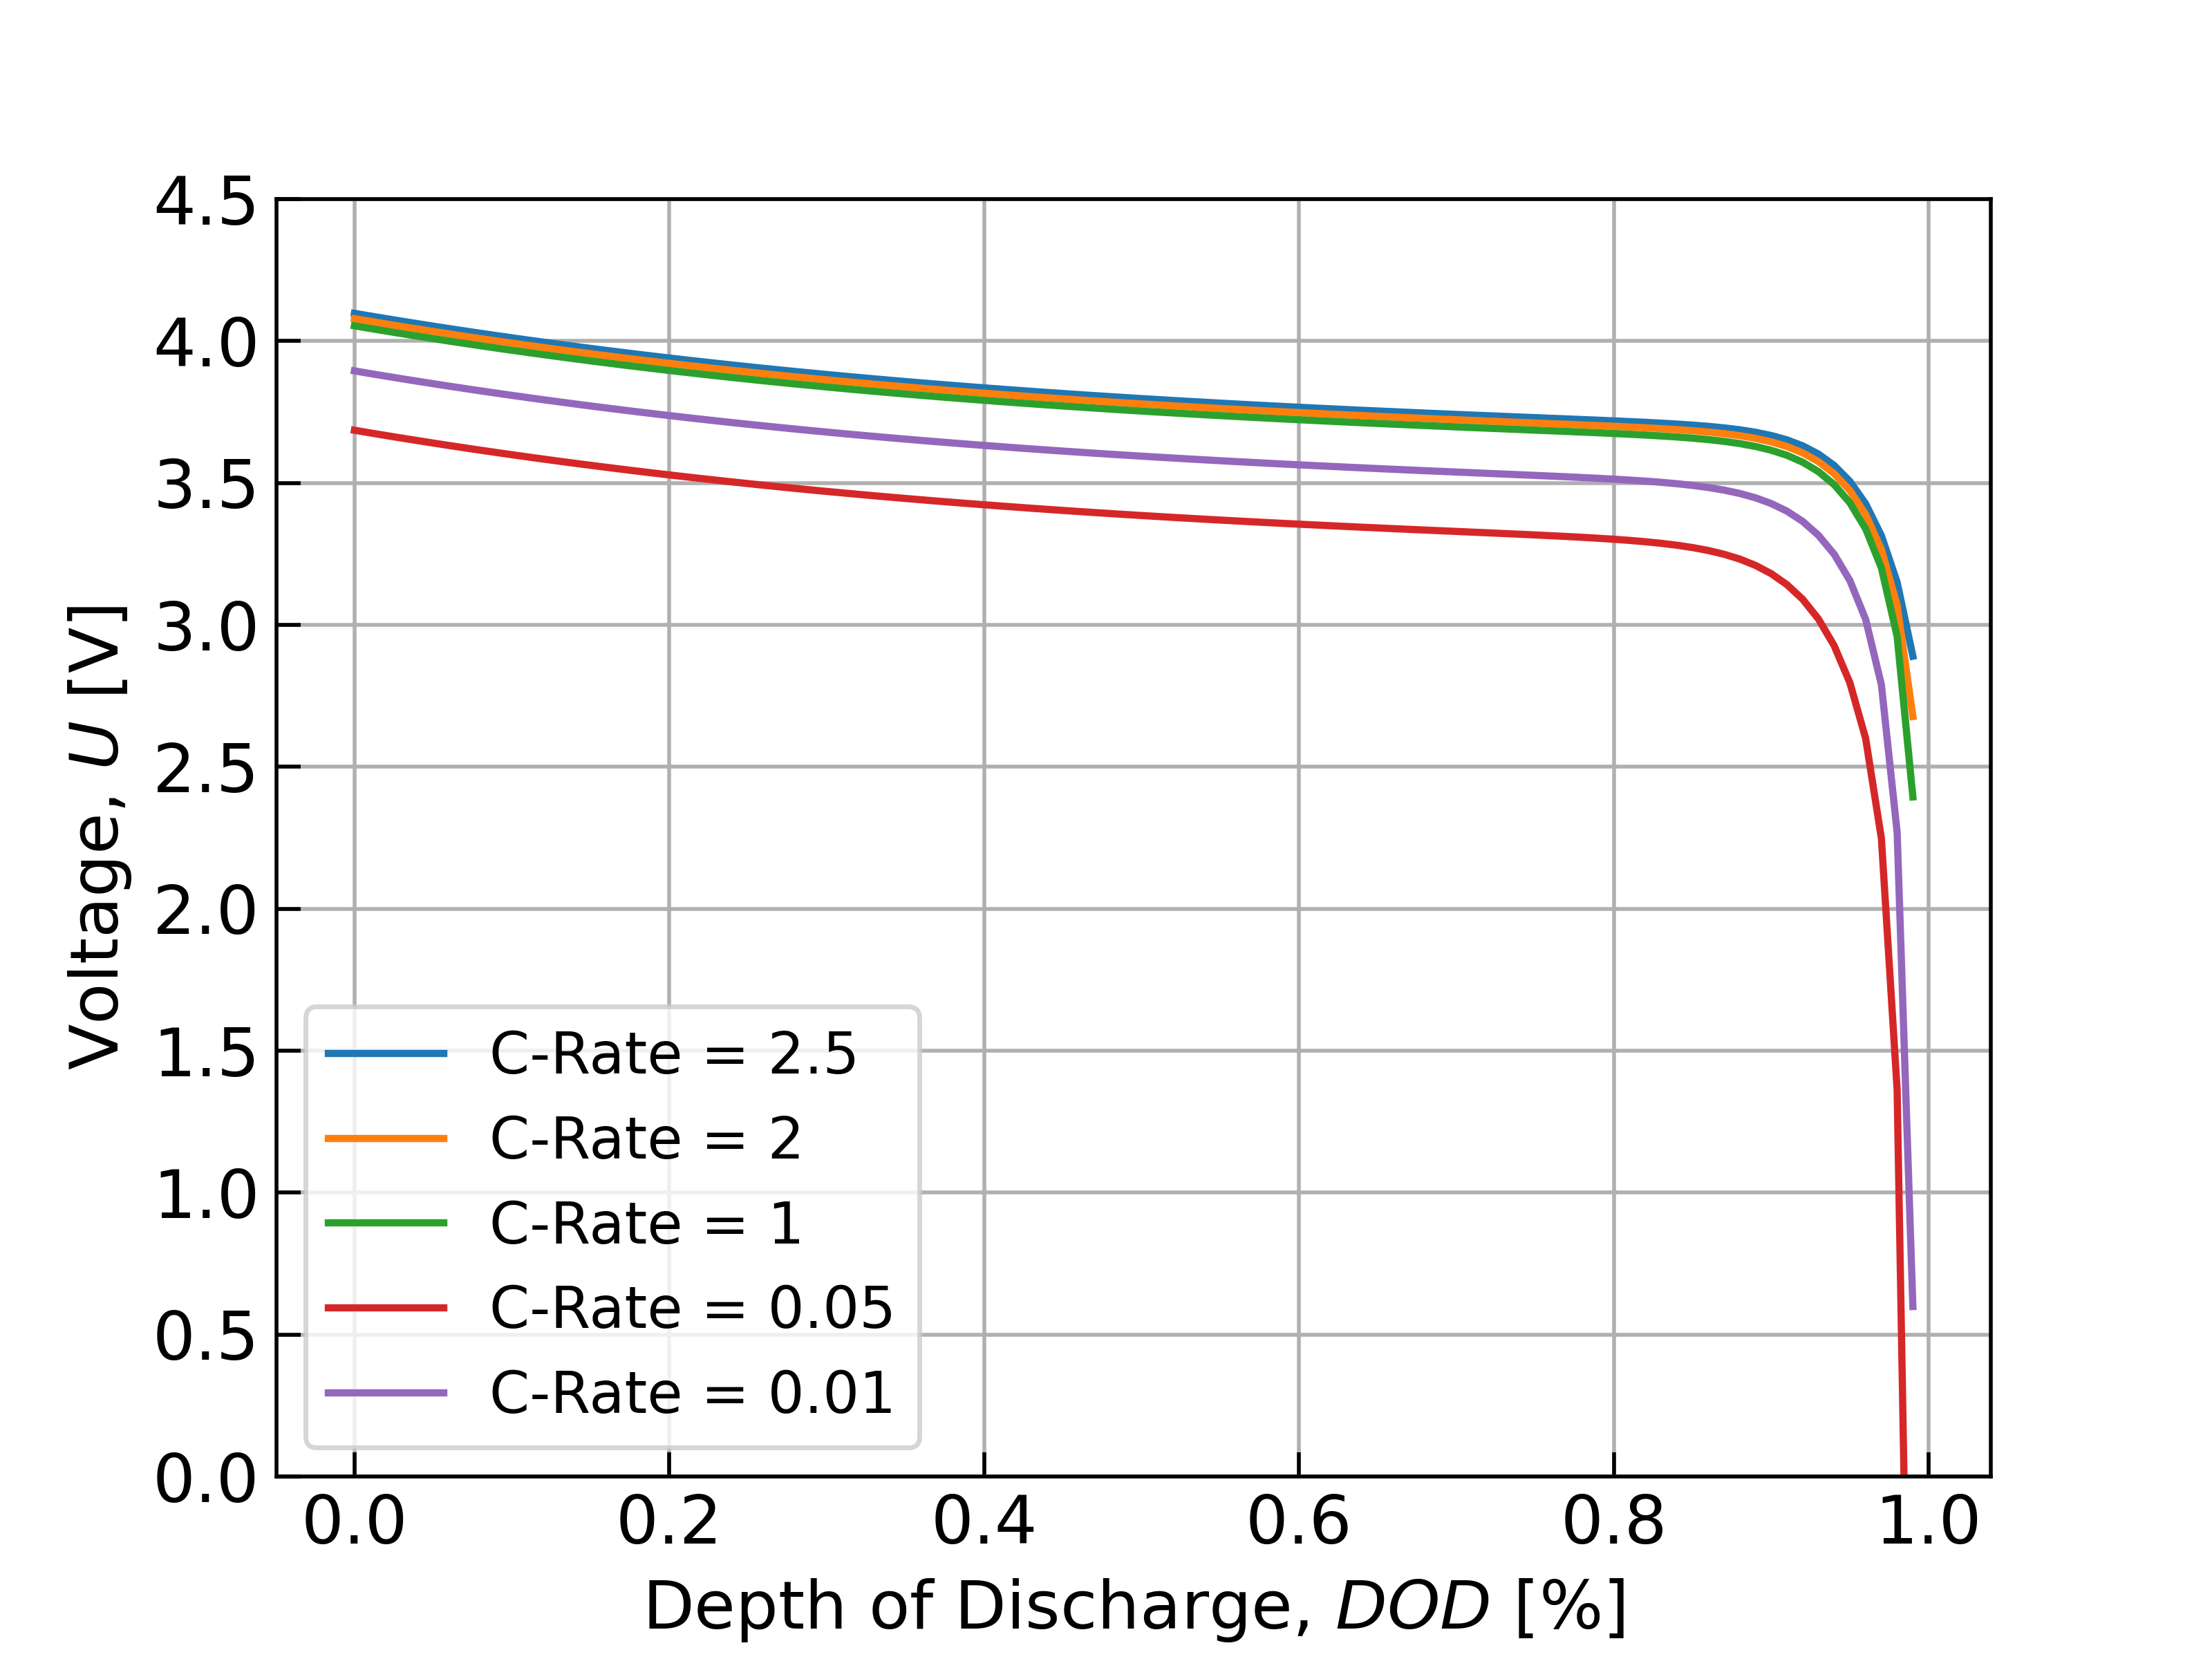
\includegraphics[width=0.5\linewidth]{figures/DODvVoltage}
    \caption{Voltage as a function of DOD per C-Rate}
    \label{fig:vvsdod}
    \end{figure}

From \Cref{fig:vvsdod}, it can be retrieved how, as discussed before, the voltage drops with the discharging of the battery.
In particular, this effect is severe at a DOD between $80\%$ and $100\%$.
This drop results in a severe loss of power, thus it is advisable to not let the battery cell reach this level.
Furthermore, as it will be discussed in \Cref{degr},
reaching this stage of discharge causes permanent damage, degrading the battery and shortening its life span.
Lastly, in the plot,
the voltages are plotted for each C-Rate, and it can be seen that for very low C-Rate values, the voltages drop as well,
thus, it is necessary to also take this effect into account.

\subsection*{Iterative Algorithm}
As it has been just described, the voltage of a battery depends on its state of charge as well.
Thus,
it is possible to create an iterative algorithm \cite{bosspaper}
that computes the power at each time step taking into account also the voltage changes.
The current SOC and nominal capacity of the battery pack are taken as input.
Subsequently, an iterative process starts to determine the actual voltage of the battery.
The voltage that the battery can provide at each time instance of the mission profile has been plotted in \Cref{fig:vol}.

\begin{minipage}{0.45\linewidth}
    \begin{figure}[H]
    \centering
    
\includegraphics[width=0.9\linewidth]{figures/VvTime}
    \caption{Battery pack voltage as a function of time}
    \label{fig:vol}
    \end{figure}
\end{minipage}
\begin{minipage}{0.45\linewidth}
    \begin{figure}[H]
    \centering
    
\includegraphics[width=0.9\linewidth]{figures/SOCvTime}
    \caption{Battery SOC as a function of time}
    \label{fig:soc}
    \end{figure}
\end{minipage}


It is visible how the voltage decreases with time, following the previously discussed relation with SOC; however, it is important to notice that for the current battery configuration,
the voltage is always above the required one from the engines of 710 V,
thus this requirement has been satisfied.

Following the algorithm successively, it is possible to calculate the SOC as a function of time as well.
To do so, it is necessary to calculate the actual capacity of the battery $C_\text{act}$.
As well as the capacity of the battery, which is a function of the voltage, also drops with time.
Hence, the new one can be estimated with the following equations.
\begin{equation}
    C_\text{act} = r_c \cdot C_\text{nom}
\end{equation}
Where $r_c$ represents the relative capacity and can be obtained as a function of time from \cite{bosspaper}.
After retrieving this parameter, the last step of the iteration can be performed,
and the battery charge as a function of time can be calculated.
This is done through the following integration:
\begin{equation}
    \text{SOC}(t) = \text{SOC}_\text{start} -  \int_{0}^{T} \frac{I}{C_\text{act}},dt
\end{equation}

To complete this calculation, an initial condition for the SOC needs to be set.
As seen before, and as it will be discussed in \Cref{degr},
the best operating range for a battery is between SOC of $20\%$ and $80\%$,
thus $S_\text{start}$ has been set to $80\%$.
Integrating the whole mission profile leads then to the generation of \Cref{fig:soc}.
\todo{Make the SOC graph $y$-axis go from 0 to 100 with ylim}

From the plot, the battery discharge pattern can be seen over the whole mission profile.
It is immediately noticeable that the most energy-consuming phase is the vertical take-off,
since the battery percentage drops by $14\%$ in roughly 4 minutes.
This is sensible; as in the take-off, all the lift is generated by the propellers,
thus the highest power is required, leading to this peak in consumption.
It can then be seen how the climb and especially the cruise are very efficient phases.
This is because the motors have to spin at a lower rate as the wings generate the majority of the required lift.
It is noticeable, particularly, how only $14\%$ of the battery energy is used during a cruise phase lasting 20 minutes.
After this, a plateau can be seen;
as during the descent, the engines are set to a very low power setting since a loss in height is required.
Lastly, another peak in energy consumption can be noticed during landing; similar to the take-off, the motors will have to spin at very high rotational speeds to have a controlled descent.
Furthermore, one thing that can be immediately seen from \Cref{fig:soc} is how only $40\%$ of the total battery capacity is used,
this means that the range could be increased further.
In particular, keeping the battery SOC between $20\%$ and $80\%$, the SOC for the new mission profile can be plotted:

\begin{figure}[H]
    \centering
    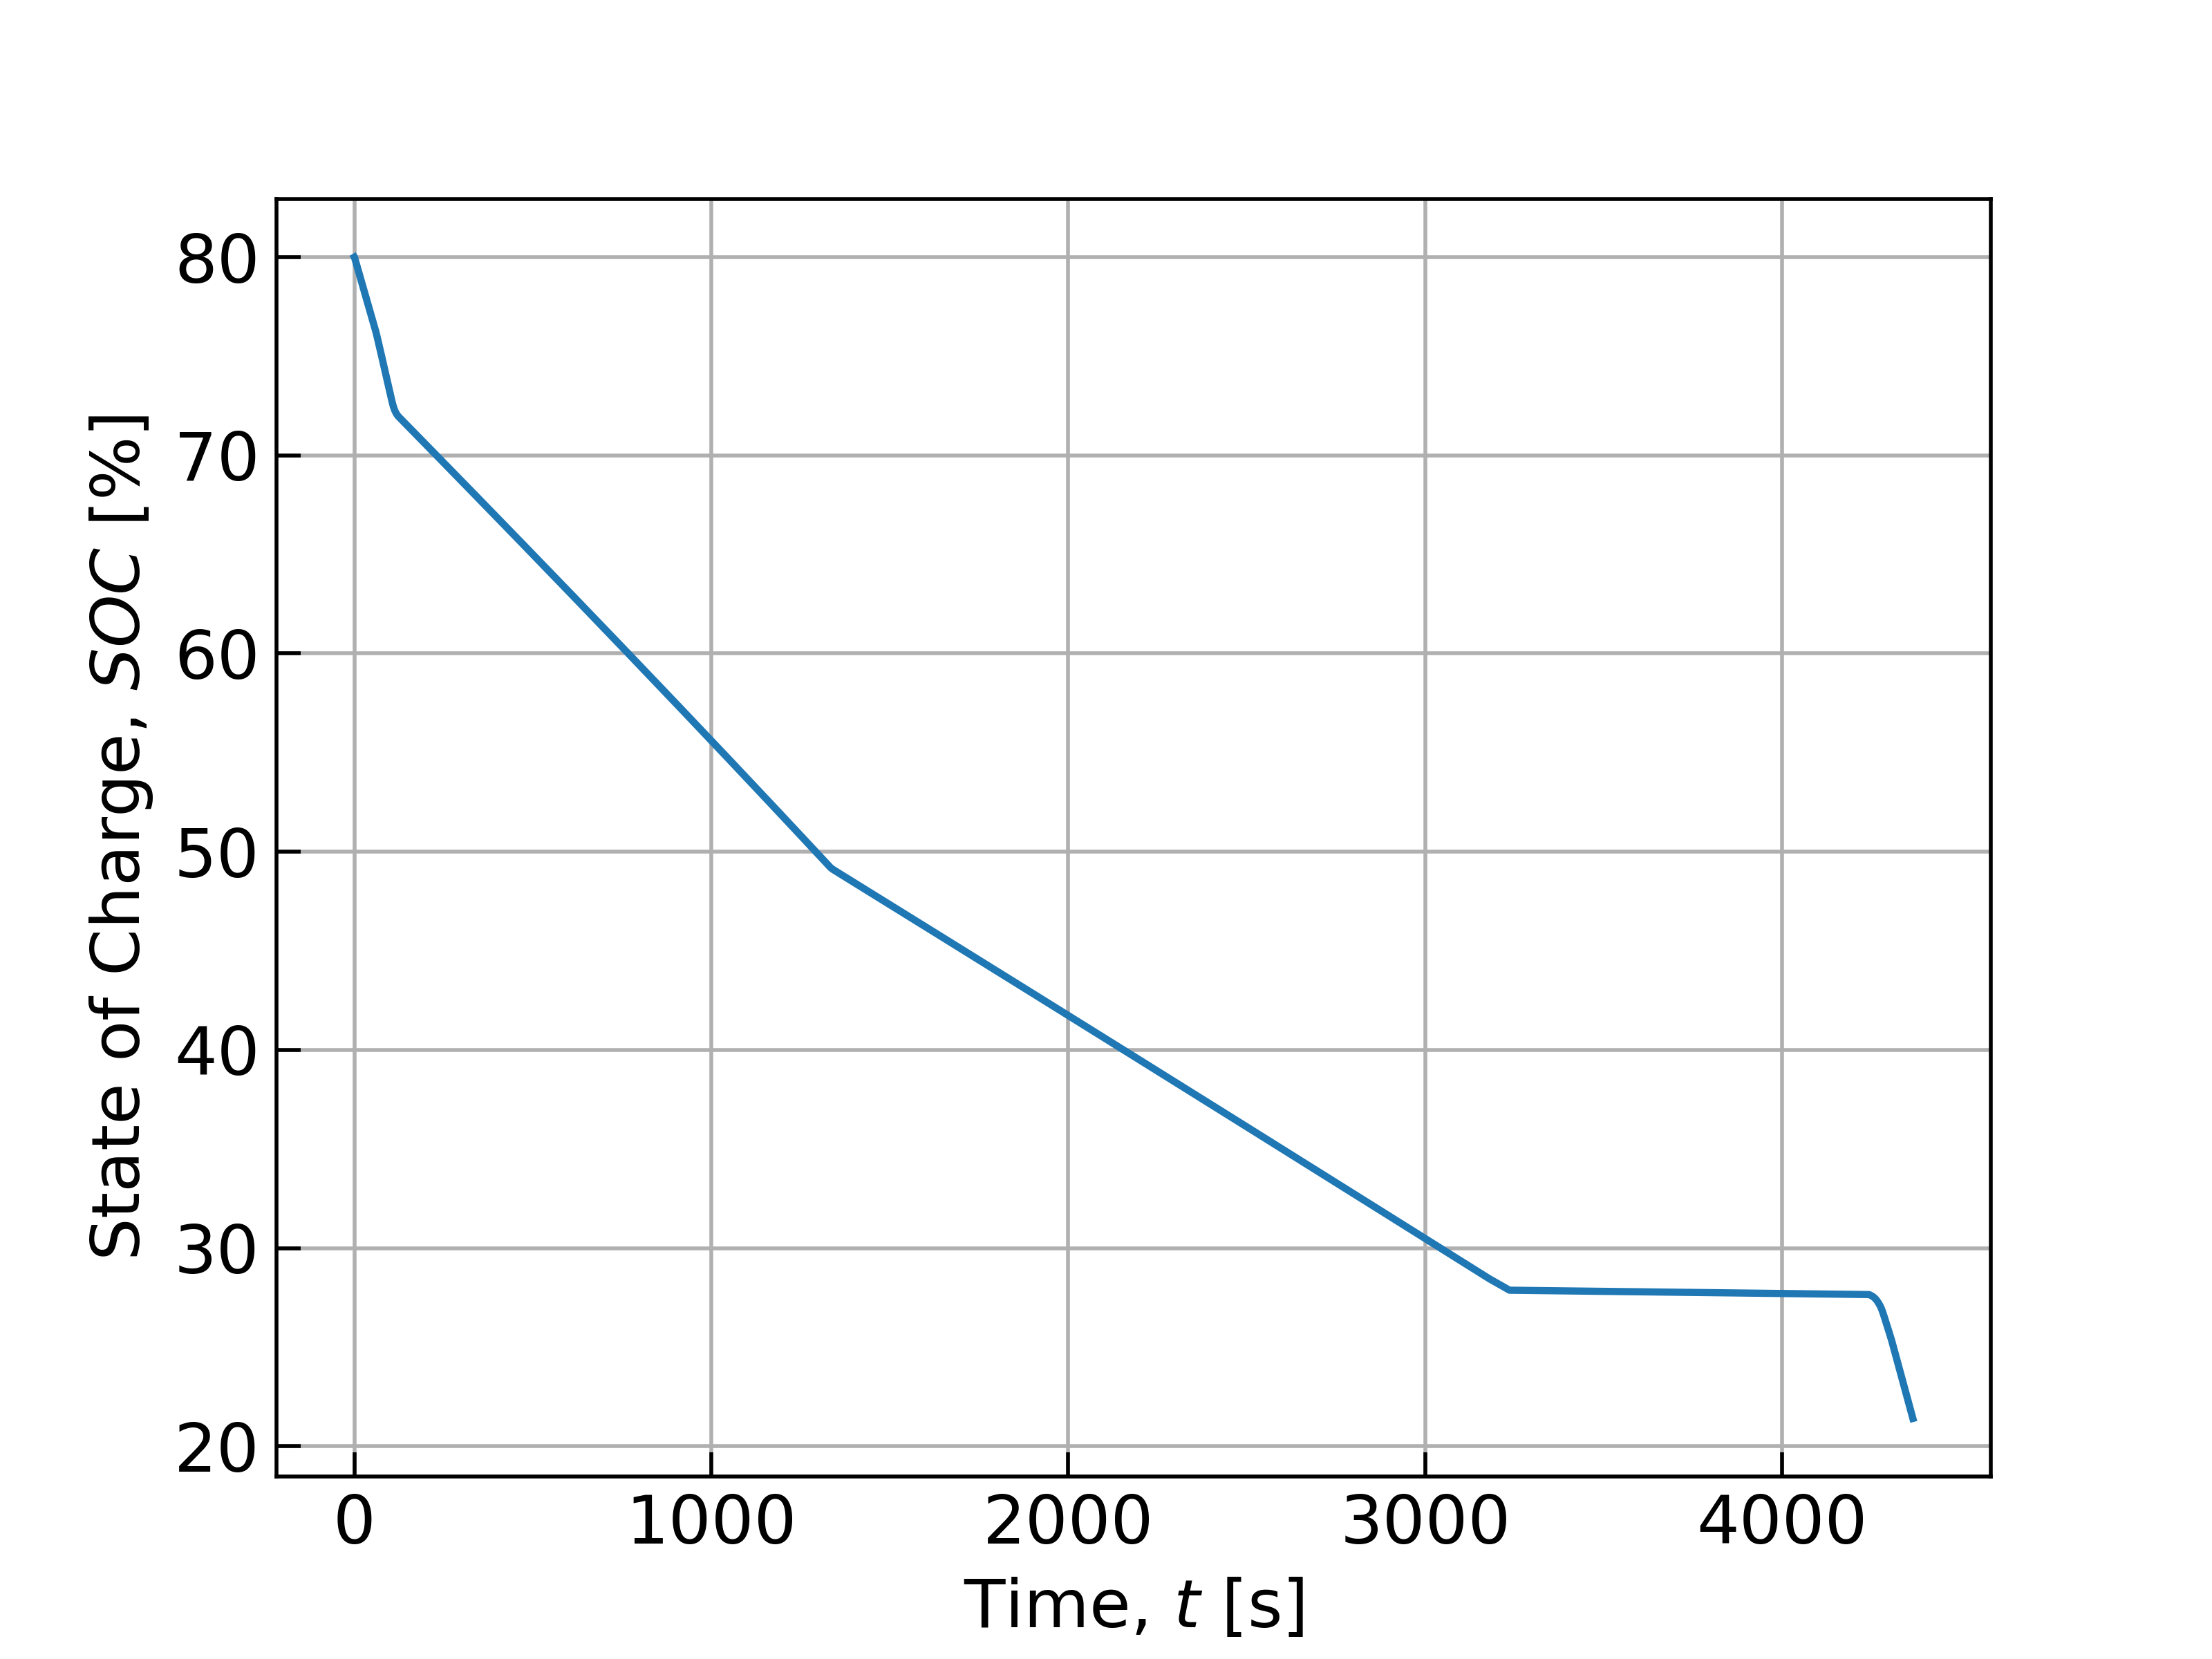
\includegraphics[width=0.5\linewidth]{figures/SOCvTime_2}
    \caption{SOC over time for the new mission profile}
    \label{fig:SOC2}
\end{figure}

Since the cruise speed does not vary and the cruise time is known, the new range is calculated to be 220 km.
This means that as discussed in \Cref{sec:Market_Segmentation} the eVTOL would be able
to reach more destinations in the contest of inter-urban mobility.
Lastly, the C-rate and the current as a function of time can be plotted as well.
For verification of the model purposes, the two curves should have the same shape since they are linearly proportional.
Furthermore, the C-Rate plot it is crucial to control the degradation of the battery,
as really high C-Rates lead to heat generation.
The two plots can be seen in the \Cref{fig:cur,fig:c-}.
As previously mentioned, the two plots have the same shape as respected.
Furthermore, the C-Rate shows peaks at the take-off due to the high power consumption,
however, it never peaks too much, limiting degradation.

\begin{minipage}{0.45\linewidth}
    \begin{figure}[H]
    \centering
    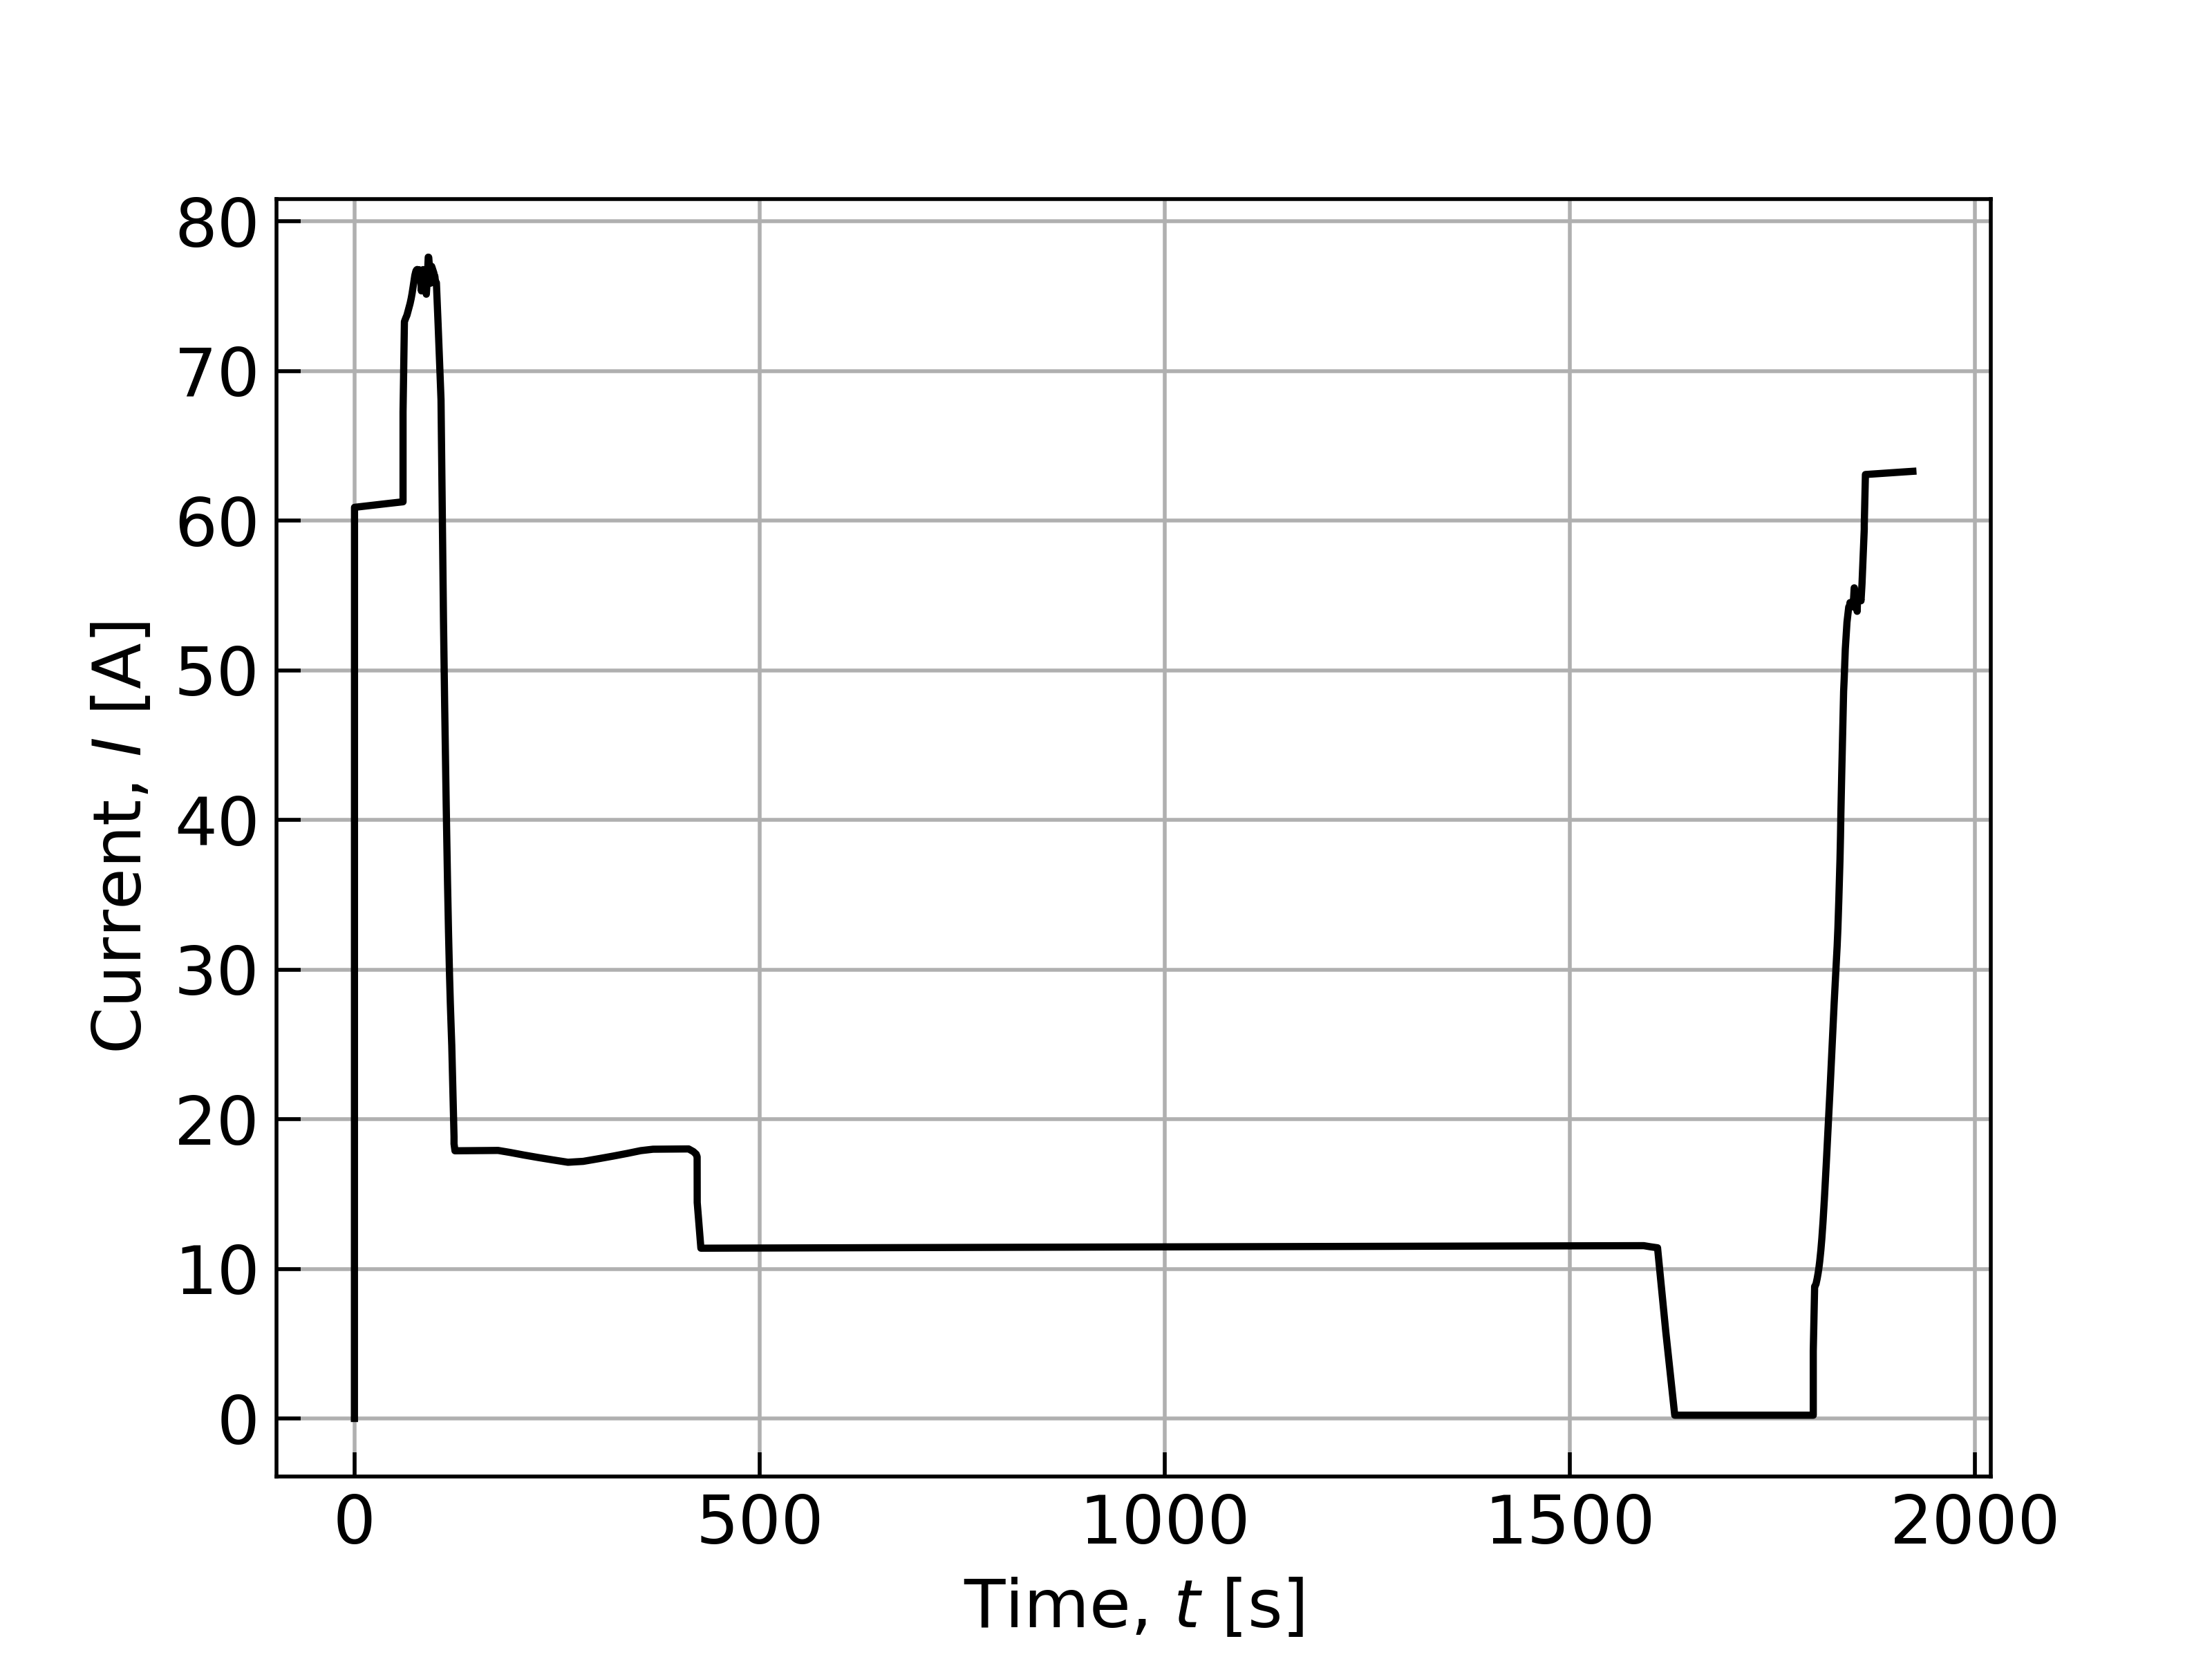
\includegraphics[width=0.9\linewidth]{figures/current}
    \caption{Current as a function of time}
    \label{fig:cur}
    \end{figure}
\end{minipage}
\begin{minipage}{0.45\linewidth}
    \begin{figure}[H]
    \centering
    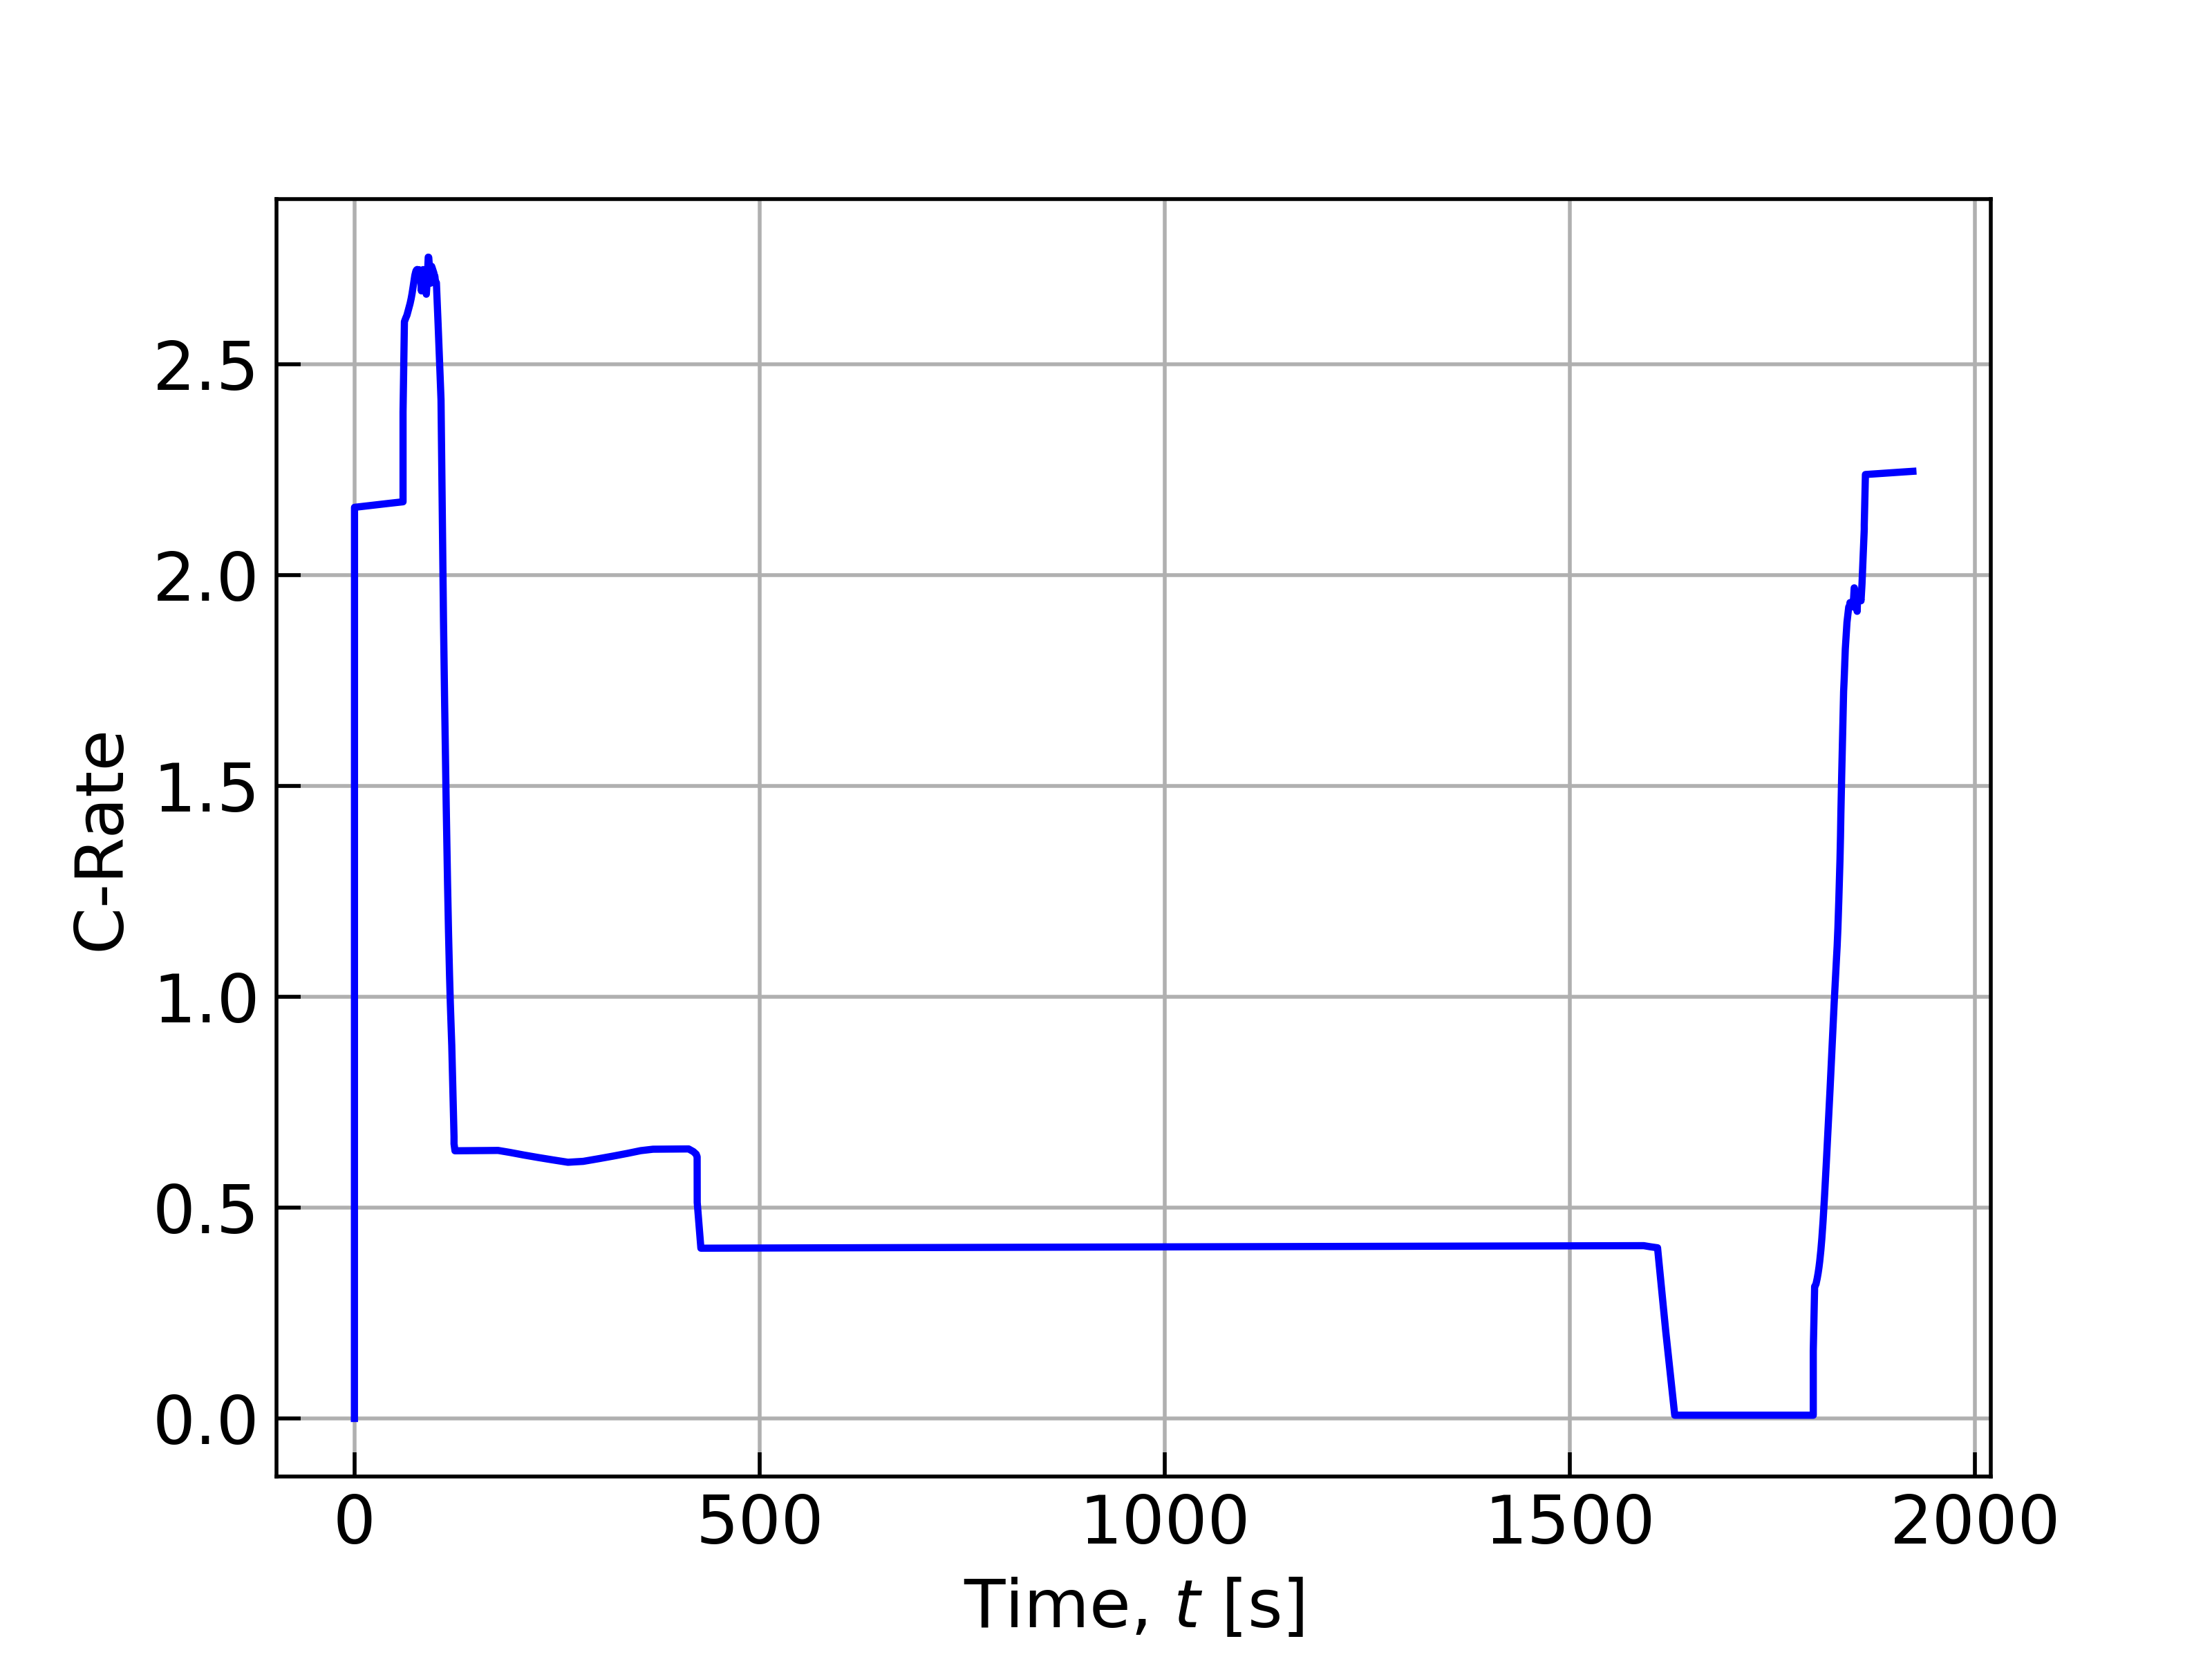
\includegraphics[width=0.9\linewidth]{figures/C-Rate}
    \caption{C-Rate as a function of time}
    \label{fig:c-}
    \end{figure}
\end{minipage}

\section{Battery Design}
\label{sec:batt_des}
In the previous sections,
all the battery cell parameters and how they vary with time, thus with SOC, have been defined and discussed.
Building upon that, it is now possible to analyze the final battery pack configuration.
Firstly, the type of cells composing the pack needs to be chosen.
Currently, the three most deployed cell types for electric vehicles are pouch, cylindrical and prismatic.
The different configurations can be seen in \Cref{fig:pouch}.

\begin{figure}[H]
    \centering
    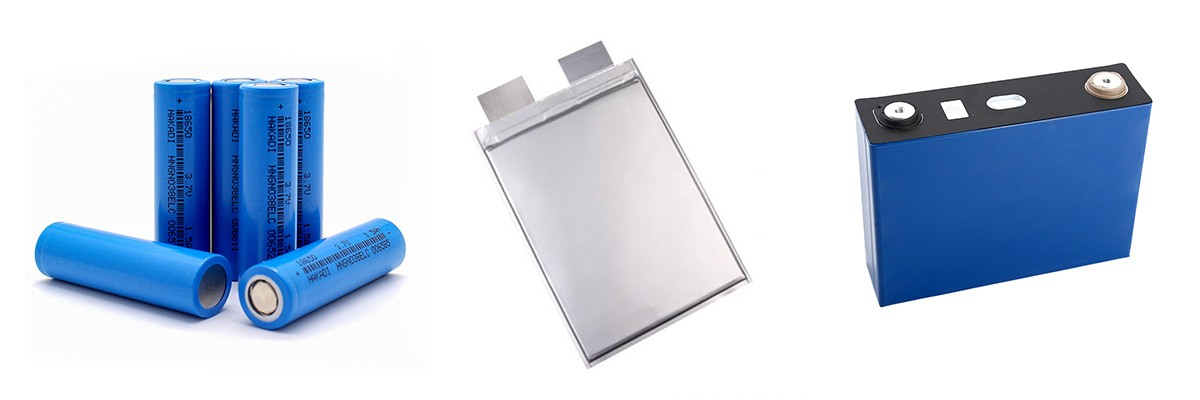
\includegraphics[width=0.5\linewidth]{figures/celltypes}
    \caption{Equivalent circuit of a battery cell discharge model}
    \label{fig:pouch}
\end{figure}

Starting from cylindrical cells, they are the most used cell type in the automotive industry.
This is because they are characterised by high energy densities
while being structurally strong and easy to cool due to their low dimensions.
On the other side, pouch cells are mechanically sensitive,
since they do not have a rigid structure covering them; thus the probability of accidental damages increases, which leads to weight savings.
Additionally, thermal management is more complicated due to the swelling of the cells during usage.
Lastly, the prismatic cells,
have great mechanical properties and energy densities.
However, their dimension is larger than the other two options,
which limits the applicability of this project as the space in the nacelle is very limited.
After a careful evaluation, the cylindrical cells have been chosen.
Mainly for their dimensions, ease of thermal management,
and the mechanical properties that give this technology an edge over pouch cells in the design of the \textit{Swing}.

Once the cell type has been chosen, the cell layout is needed.
It has been decided to use six different battery packs, each of which powers one engine.
The voltage $U_\text{sys}$ is 710 V,
while the required capacity has been determined to be 28 Ah, using \Cref{capa}.
In order to obtain these results, cylindrical cells with the following properties have been considered:
\begin{itemize}
    \item $U_\text{nom} = \qty{3.7}{V}$
    \item $C_\text{nom} = \qty{7000}{mAh}$
\end{itemize}
To increase the voltage, cells need to be connected in series,
meaning that the anode of one cell connects to the cathode of another.
When connecting cells in this way, the total voltage can be calculated as:
\begin{equation}
    U_\text{tot} = N_\text{series} \cdot U_\text{cell}
\end{equation}
Being $U$ the voltage and $N_{series}$ the number of cells in series.
Inverting this formula, it can be found that in order to reach a $U_\text{tot} = \qty{710}{V}$,
192 cells connected in series are thus needed.
Once the voltage requirements are met, the capacity requirement needs to be analysed as well.
In order to increase capacity, cells need to be connected in parallel.
Similarly to the voltage, the total capacity can be computed as:
\begin{equation}
    C_\text{tot} = M_\text{parallel} \cdot C_\text{cell}
\end{equation}

Having each cell a capacity of 7 Ah, it can be found that four cells connected in parallel are needed to reach the capacity of 28 Ah.
The pack could now be designed in one single module with the following configuration 192S x 4P.
However, a single-module design has several disadvantages.
Mainly,
in case of minor defects, can lead
to changing the whole battery in addition to the fact that the battery becomes less accessible.
Opting for a multiple-module configuration, helps with the modularity of the design,
leading to only certain parts of the battery being replaced if needed.
Each module has been designed to have twelve cells in series and 4 in parallel, 12S x 4P configuration.
Then sixteen modules are connected in series to reach the voltage requirement.
A visualisation of each module has been produced in \Cref{fig:moduleu}.

\begin{minipage}{0.6\linewidth}
    \begin{figure}[H]
    \centering
    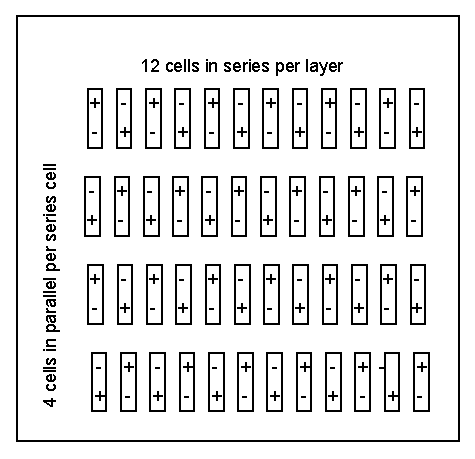
\includegraphics[width=0.95\linewidth]{figures/batterypack design.pdf}
    \caption{Configuration of each battery module}
    \label{fig:moduleu}
    \end{figure}
\end{minipage}
\begin{minipage}{0.4\linewidth}
    \begin{figure}[H]
    \centering
    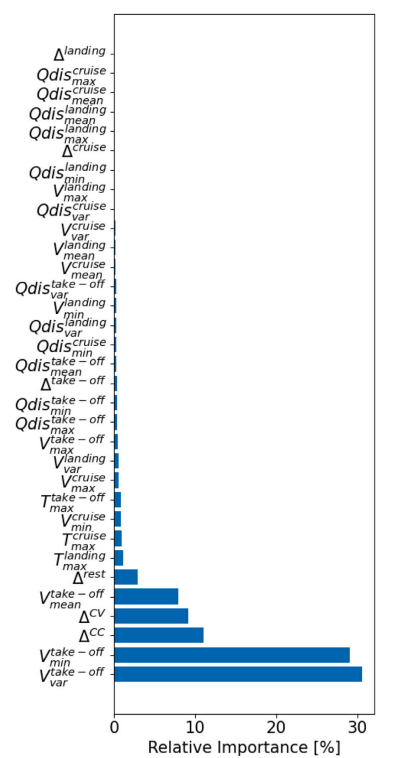
\includegraphics[width=0.95\linewidth]{figures/marilena}
    \caption{Relative importance of battery parameters on degradation \cite{batteryhealth}}
    \label{fig:marilena}
    \end{figure}
\end{minipage}

\subsection{Battery Degradation and Health Estimations}\label{degr}
One of the main areas of concern when developing an electric power vehicle is battery health management.
This is even more relevant in the case of eVTOLs,
where the discharge rates are very high during the take-off and landing phases,
impacting the overall lifespan of a pack~\cite{batteryhealth}.

The process that decreases the capacity of a lithium-ion battery is also called Solid Electrolyte Interphase (SEI) degradation.
SEI is a thin layer of organic material that forms on the anode of the battery.
Its main characteristics are facilitating the passage of ions, as well as protecting the anode from any decomposition.
This thin layer, however, damages with time,
resulting in decreased battery capacity, and an increase in internal resistance\cite{tatz}.
Knowing the degradation process, it is now useful to understand which parameters influence it,
thus estimating how to limit it to increase the lifespan of the battery pack.
These parameters have been studied in \cite{batteryhealth}.
Here a machine learning predictive model has been developed,
thus the State of Health (SOH) of batteries has been estimated,
indicating the effect of each flight phase on the degradation of the capacity.
The algorithm used in \cite{batteryhealth} has been trained on public data for different mission profiles for the Airbus Havana eVTOL.
From the results presented by the paper, visible in \Cref{fig:marilena}~\cite{batteryhealth},
it has been found that the voltage variance during take-off ($\Delta U_\text{take-off}$) has the highest impact,
followed by the minimum voltage during take-off and charging phase duration.

These results can be explained by the fact
that during the take-off, the battery has to provide very high power coupled with high C-Rates, as can be seen in \Cref{fig:c-}.
The charging time instead is a function of the voltage and current.
The faster the charging, the higher the power rating, which leads to batteries heating up,
causing permanent damage to the SEI layer, and decreasing capacity drastically.
Lastly, as mentioned before,
the SOC is another parameter that must be taken into account when dealing with SOH management.
It has been found by \cite{Li_2021},
Li-Ion batteries are particularly sensitive when operating and charging close to the cut-off voltage.
This happens when going above a SOC of $80\%$ or below $20\%$.
For example, for a specific battery, it has been found that charging fully and going then to SOC of $0\%$ in each cycle
would lead to only 1000 cycles of life span.
On the other side, charging between SOC of $40\%$ and $70\%$ leads to a life span of 2000 cycles~\cite{Li_2021}.
For this reason, it has been decided to size the battery such that can meet the range requirement,
operating only between the optimal SOC of $20\%$ to $80\%$.

Once these have been defined, the total battery life span for the eVTOL design can be estimated.
In order to do so, the power per cell during take-off has been calculated:
\begin{equation}
    P_\text{cell} = I_\text{cell} \cdot V_\text{cell}
\end{equation}
\begin{equation}
    I_\text{cell} = \frac{I_\text{pack}}{m_\text{parallel}}
\end{equation}
\begin{equation}
        P_\text{cell} = \qty{51}{W}
\end{equation}
This calculation results in a power per cell of 51 W,
which is very similar to the one of the Havana of 54 W~\cite{Li_2021}.
Furthermore, the nominal voltage for the cells is identical at 3.7 V,
making a comparison a reasonable method to estimate the life-cycle.
From the database, it can thus be found that the battery life span for this kind of battery averages around 800 cycles.
It is, however, important to note
that the end of life is defined at the point the pack reaches the $85\%$ of its nominal capacity.
This is a high limit, but necessary for safety reasons, especially during the take-off phase,
the battery needs to be able to provide enough voltage without drops.

Lastly, the charging power rating for the battery has to be determined.
In particular, it has been decided to use a power rating of 250 kW,
in this way the 120 kWh battery could be completely charged in less than 30 minutes.
This power rating has been decided upon research on ground electric vehicles.
As an example,
Tesla superchargers use the same rating~\cite{tesla1}
and their batteries are designed to last at least 1500 charging cycles.
This indicates
that this is a feasible rating that puts a compromise between low charging time and battery capacity conservation.

\subsection{Battery Cooling}
From \Cref{degr} it is clear that keeping the battery at an optimal temperature is fundamental during operations.
If the temperature increases too much,
the battery will not deliver the expected power and will be permanently damaged, leading to a decrease in the lifespan.
From the mission profile analysis,
it is clear that the battery will deliver the highest power during vertical off and descent,
thus in these phases, there will be the highest heat generation, leading to a severe increase in temperature.
To avoid this, air-cooling could be adopted.
However, during the vertical ascent, the airspeed is very low.
Even the stream of the propeller would not be optimal to keep the batteries at a controlled temperature.
Furthermore, having additional openings in the aircraft will create additional drag during the cruise,
reducing aerodynamic performances.
For this reason, it has been decided to opt for a liquid-cooling thermal management system,
similar to Joby aviation \cite{joby}.
The cooling system will be composed of a pump and several tubes containing coolant
that will tangentially touch each cylindrical cell,
extracting the heat from the cell.
An exemplification of this can be seen in \Cref{fig:vis} \cite{coolingpic},
while a diagram of the heat extracting system has been produced in \Cref{fig:ciao}.

\begin{minipage}{0.45\linewidth}
    \begin{figure}[H]
    \centering
    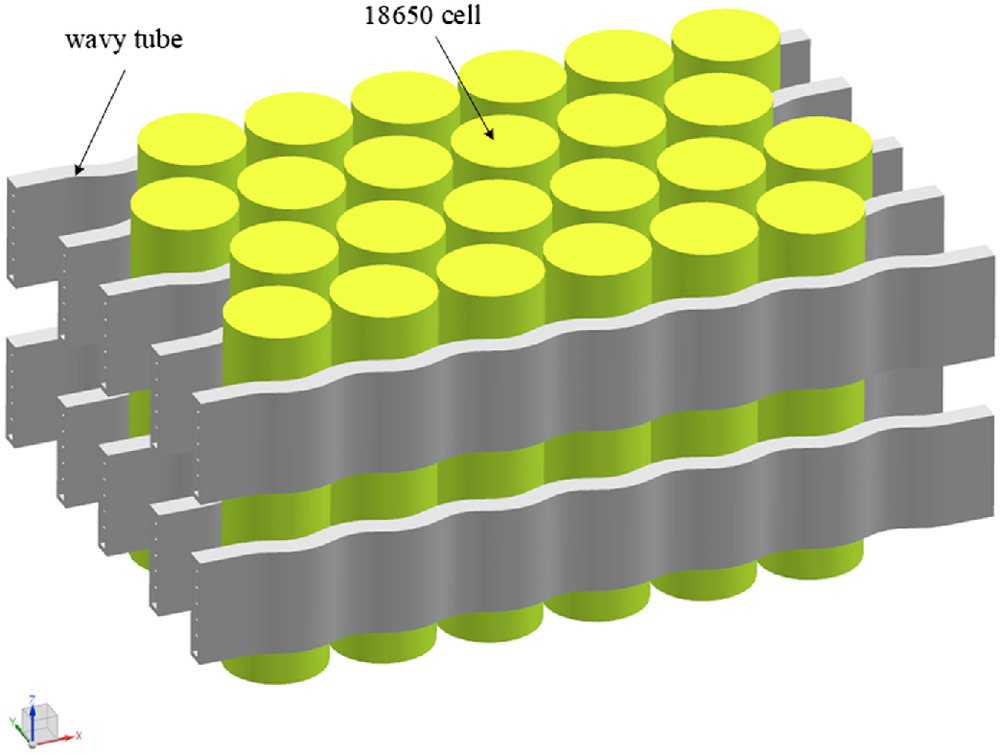
\includegraphics[width=0.5\linewidth]{figures/figure5 (1)}
    \caption{Cylindrical cells liquid cooling \cite{coolingpic}}
    \label{fig:vis}
    \end{figure}
\end{minipage}
\begin{minipage}{0.45\linewidth}
    \begin{figure}[H]
    \centering
    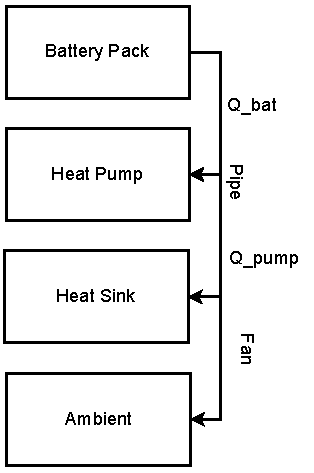
\includegraphics[width=0.5\linewidth]{heat_pumps.pdf}
    \caption{Heat pump scheme}
    \label{fig:ciao}
\end{figure}
\end{minipage}\\
Lastly, it is important to note that the battery capacity is enough to account for the consumption of the cooling system without drastically compromising the range.
\section{Design Summary and Recommendations}
\label{sec:eps_concrec}
The design of the battery has been divided into many steps with several layers that might be hard to understand at first sight, thus this section aims to give a clear overview of the final results.
\Cref{fig:overvieww} illustrates the complete battery design from a top-level perspective showcasing how each pack is made and all its layers.
In addition to this, \Cref{tab:batt_table} presents the final values for many parameters of the aircraft batteries.

\begin{figure}[H]
    \centering
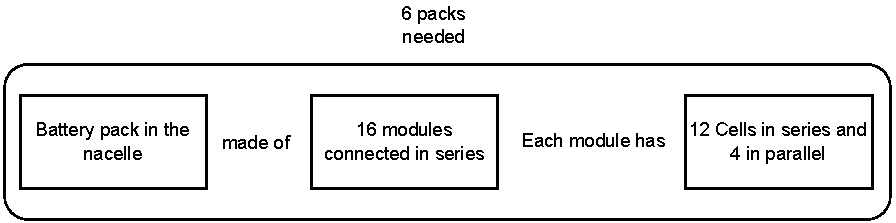
\includegraphics[width=0.8\linewidth]{figures/summary_battery.pdf}
    \caption{Complete battery system overview}
    \label{fig:overvieww}
\end{figure}




\begin{table}[htpb]
\centering
\caption{Battery parameters summary}
\label{tab:batt_table}
\begin{tabular}{cccccc}
\toprule
\textbf{$N_{cells}$ {[}-{]}} & \textbf{$N_{tot}$ {[}-{]}} & \textbf{$w_{cell}$ {[}-{]}} & \textbf{$w_{tot}${[}kg{]}} & \textbf{$E_{pack}$ {[}kWh{]}} & \textbf{$E_{tot}$ {[}kWh{]}} \\ \hline
\midrule
768                              & 4608                          & 0.09                    & 400                  & 20000                         & 120                    \\ \hline
\bottomrule
\end{tabular}
\end{table}


Lastly, as the field of battery development is currently a thoroughly studied field, some recommendations for further development are necessary. In this paper, standard Li-Ion cells have been considered, however, new developments of new types of cells are being developed. For instance, particular attention shall be paid to the developments of lithium-sulfur \cite{sulphure} and solid-state batteries\cite{solidstate}, which can offer overall better performances, increasing capacity and thus reducing weight. In addition to this, companies like Tesla should be paid, as they are developing new highly efficient cylindrical cells (Tesla 4680) \cite{Tesla} that are very close to the state-of-the-art energy density of the current technologies.